\sect{5. How to play}

You and your partner drive the pursuit car of \textbf{Chase H.Q.}, the special investigation unit. In each of the five stages a criminal is escaping in his car. Nancy tells you by radio who he is at the start of the stage. Then:

\begin{enumerate}
\item \textbf{Catch up with him.} The \texttt{DISTANCE} counter shows how far ahead he is, and you have \textbf{60 seconds}. Overtake the traffic and stay on the road.
\item When he comes into view, \texttt{SIGHTING OF TARGET VEHICLE} appears, the \textbf{siren} starts, and the clock goes back to \textbf{60 seconds}.
\item \textbf{Ram his car} again and again. Each ram drains the damage meter on the left of the road; after \textbf{20 rams} he gives up, pulls over and is arrested.
\end{enumerate}

\begin{figure}[H]
\centering
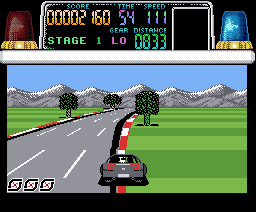
\includegraphics[width=0.48\textwidth]{../img/stage1.png}\hfill
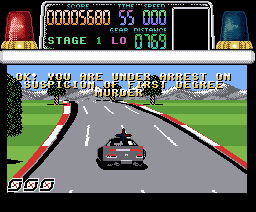
\includegraphics[width=0.48\textwidth]{../img/arrest.png}
\caption{Left: the chase in the first stage. Right: the arrest.}
\end{figure}

\textbf{On the road.} Crashing into another car or into something at the roadside (trees, signs, fences) spins you round and slows you down. Off the road the car shakes and loses speed. The road goes through tunnels, and sometimes it splits in two. If you drive too slowly for too long, your partner complains.

\textbf{The radio.} The line under the panel shows what is said on the radio, letter by letter, with the face of whoever is speaking: Nancy, your partner or the criminal.

\textbf{Time up and continue.} If the clock reaches zero, \texttt{TIME UP} appears. If you have credits left, \texttt{CONTINUE THIS MISSION} counts down from 10: press \textbf{GEAR} before it reaches 0 to go on with 60 seconds and three turbos, but the criminal's car is repaired. You have \textbf{two credits} per game. Without credits, or if you let the count run out, the game is over.

\begin{figure}[H]
\centering
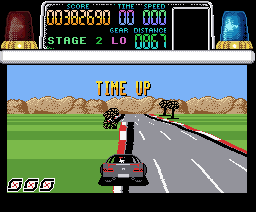
\includegraphics[width=0.48\textwidth]{../img/timeup.png}\hfill
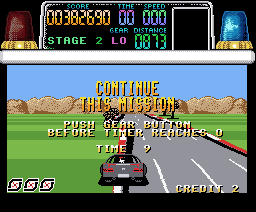
\includegraphics[width=0.48\textwidth]{../img/continue.png}
\caption{Left: the clock has run out. Right: the chance to continue.}
\end{figure}

% ==================================================================
\sect{6. The status panel (HUD)}

\begin{figure}[H]
\centering
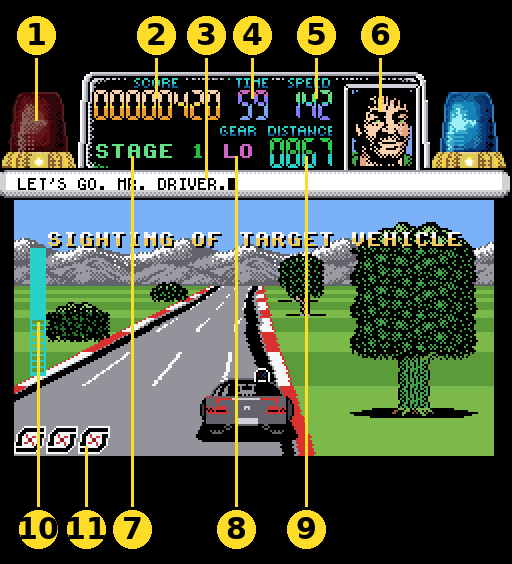
\includegraphics[width=0.9\textwidth]{img/hud.png}
\caption{The panel at the top of the screen, and what you see on the road.}
\end{figure}

\begin{tabularx}{\textwidth}{@{}cp{3.1cm}X@{}}
\toprule
\textbf{\tNo} & \textbf{\tElement} & \textbf{\tTellsYou}\\
\midrule
1 & Sirens & The two police lights. They flash while the siren sounds, once the criminal is in sight.\\
2 & \texttt{SCORE} & Your score.\\
3 & Radio & What is said on the radio, letter by letter.\\
4 & \texttt{TIME} & Seconds left.\\
5 & \texttt{SPEED} & Your speed in km/h.\\
6 & Face & Who is speaking on the radio: Nancy, your partner or the criminal. Static when the radio tunes in.\\
7 & \texttt{STAGE} & The stage you are playing, 1 to 5.\\
8 & \texttt{GEAR} & The gear you are in: \texttt{LO} or \texttt{HI}.\\
9 & \texttt{DISTANCE} & How far away the criminal is.\\
10 & Damage meter & Appears once the criminal is in sight: how much his car can still take. It drains with every ram; when it is empty, he is caught.\\
11 & Turbos & The turbos you have left in this stage.\\
\bottomrule
\end{tabularx}

% ==================================================================
\sect{7. Scoring and credits}

\begin{itemize}
\item You score points all the time while you drive: the faster, the more.
\item \textbf{Overtaking} scores too, and each car you overtake is worth more than the one before (200, 400, 600\ldots{} up to 8\,000). Crashing into a car starts the count again.
\item Every \textbf{ram} on the criminal's car scores points.
\item After the arrest you get two bonuses: \texttt{CLEAR BONUS}, \textbf{100\,000 points for each stage number} (10\,000 if you have used a credit), and \texttt{TIME BONUS}, \textbf{5\,000 points for each second left}.
\item There are no lives: you play against the clock, with \textbf{two credits} to continue.
\end{itemize}

\begin{figure}[H]
\centering
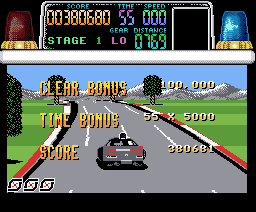
\includegraphics[width=0.48\textwidth]{../img/bonus.png}\hfill
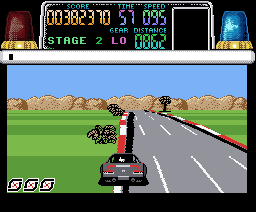
\includegraphics[width=0.48\textwidth]{../img/stage2.png}
\caption{Left: the bonuses after an arrest. Right: the second stage.}
\end{figure}

% ==================================================================
\sect{8. Tips}

\begin{itemize}
\item Change to \texttt{HI} as soon as you are moving: in \texttt{LO} the top speed is much lower.
\item Keep the turbos for when the criminal is in sight: with the turbo on, you keep more speed after each ram.
\item Overtake without touching the other cars: a crash costs speed, time and your overtaking points.
\item Stay on the tarmac: off the road you lose speed, and with it time.
\item The briefing tells you what car the criminal drives: look for it among the traffic.
\end{itemize}
